%\chapter{Problemas de Visual SLAM} \label{cap:problemavlsam}
\section{Problemas de Visual SLAM} \label{s:problemavlsam}

Actualmente las técnicas de Visual SLAM presentan algunos problemas o inconvenientes que todavía son difíciles de sortear en la práctica. En esta sección presentaremos algunos de ellos:

\subsection{Inicialización del Mapa:}

Si en Visual SLAM queremos conseguir una estimación lo más exacta posible de la posición de la cámara es necesario contar con una buena inicialización del Mapa. Se debe contar con un sistema de coordenadas globales definido, y se tomarań puntos de referencia del entorno como puntos iniciales del mapa en el sistema global de coordenadas. Utilizando este método podemos inicializar VisualSLAM en un sistema de coordenadas global en la tierra. La transformación de estos puntos iniciales al sistema de referencia global se realizará mediante homografía.

Objetos de referencia como objetos 3D también se han utilizado para obtener un sistema global de coordenadas, posiciones iniciales de la cámara son estimadas gracias al seguimiento de objetos de referencia.
En MonoSLAM por ejemplo se utilizan al menos 4 puntos 3D como objetos de referencia, y la forma del objeto se usa para mejorar el mapa.

\subsection{Ambigüedad en la escala:}

En algunas aplicaciones con Visual SLAM se necesita información de escala absoluta. Para obtener una referencia de escala absoluta se pueden utilizar zonas de la anatomía del usuario, como la cara, su mano o el propio cuerpo. En todos estos métodos se asume que entre personas la diferencia de tamaño es mínima para dichas partes del cuerpo. Se han dado otras aproximaciones como utilizar algunos de los sensores con los que ya están equipados la mayoría smartphones tales como acelerómetros, giroscopios y sensores magnéticos. Para eliminar el ruido de estos sensores se utiliza una técnica de filtro de dominio de frecuencia.

\subsection{Distorsión Rolling Shutter:}

Para conseguir una estimación de la posición de la cámara exacta, es importante considerar el tipo de shutter en la captura de la imagen. La mayoría de las técnicas de VisualSLAM asumen algoritmos \textit {global shutter}, y estos algoritmos estiman una posición de cámara para cada frame. Sin embargo existen en el mercado multitud de cámaras incluidas las RGB-D que emplean \textit {Rolling Shutter} debido a su coste. En las cámaras que utilizan el modo \textit{Rolling Shutter}, cada fila de una imagen capturada es tomada por una posición diferente de la cámara. Es obvio que es bastante complicado estimar directamente la posición de la cámara para cada fila. Se utilizará una aproximación basada en interpolación para estimar el \textit{Rolling shutter}. En algunas ocasiones se ha utilizado con éxito una función spline para interpolar la trayectoria de la cámara \footnote{https://www.premiumbeat.com/blog/know-the-basics-of-global-shutter-vs-rolling-shutter/}.

\begin{figure}[htbp]
\begin{center}
\subfigure[]{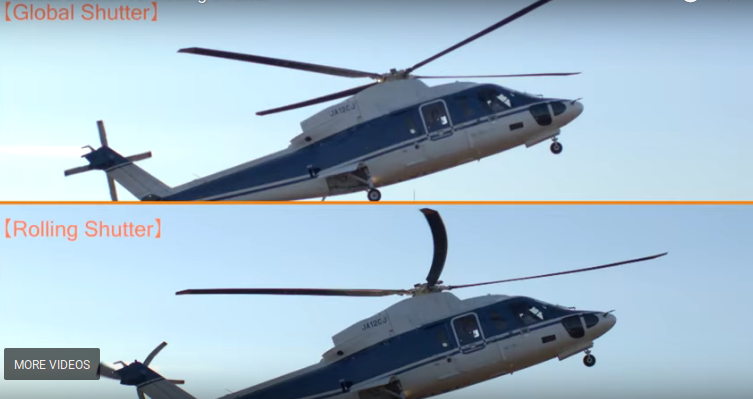
\includegraphics[height=5.0cm]{img/cap3/RollingShutter.png}}
\end{center}
\caption{Diferencias entre Global Shutter y Rolling Shutter (a)}
\end{figure}


\subsection{Dificultad para operar en entornos con pocas texturas:}

Visual SLAM utiliza el emparejamiento de píxeles o puntos característicos entre varios frames consecutivos. El emparejamiento suele fijarse en esquinas, bordes  o puntos distintivos que fácilmente podrán localizarse entre frames. Pero cuando en el entorno hay pocas texturas o presenta una alta monotonía de texturas,  el emparejamiento es difícil de realizar ya que un punto en un fotograma podría corresponder con N puntos en el siguiente fotograma y por tanto se dispararía el error de posición. Quizá este sea uno de los problemas más difíciles de solucionar con VisualSLAM
\cite{Takafumi17}.

